\documentclass[a4paper,11pt,landscape,twocolumn]{article}

\usepackage{préambule}
\usepackage{clipboard}
\usetikzlibrary{calc}

\begin{luacode}
	function print_items(points)
		for _, p in ipairs(points) do
			tex.sprint("\\item abscisse = ", p.x, ", ordonnée = ", p.y)
		end
	end

	function print_path(points)
		tex.sprint("\\draw[red,thick] ")
		for i, p in ipairs(points) do
		 	if i ~= 1 then
		 		tex.sprint(" -- ")
		 	end
		 	tex.sprint("(", p.x, ",", p.y, ")")
		end
		tex.sprint(";")
	end
\end{luacode}

\begin{document}

\directlua{
	points = {
			{ x = 1, y = 1 },
			{ x = 1, y = 2 },
			{ x = 3, y = 2 },
			{ x = 3, y = 4 },
			{ x = 2, y = 4 },
			{ x = 2, y = 5 },
			{ x = 4, y = 5 },
			{ x = 4, y = 3 },
			{ x = 5, y = 3 },
			{ x = 5, y = 5 },
		}
}

\Copy{alpha}{
	{\large \textbf{Coordonnées α :}}
	\begin{enumerate}[label={\Alph* :}]
		\directlua{print_items(points)}
	\end{enumerate}

	\vspace{2em}
	\hrule
	\vspace{2em}

	\textbf{Labyrinthe α :} \vspace{1em}

	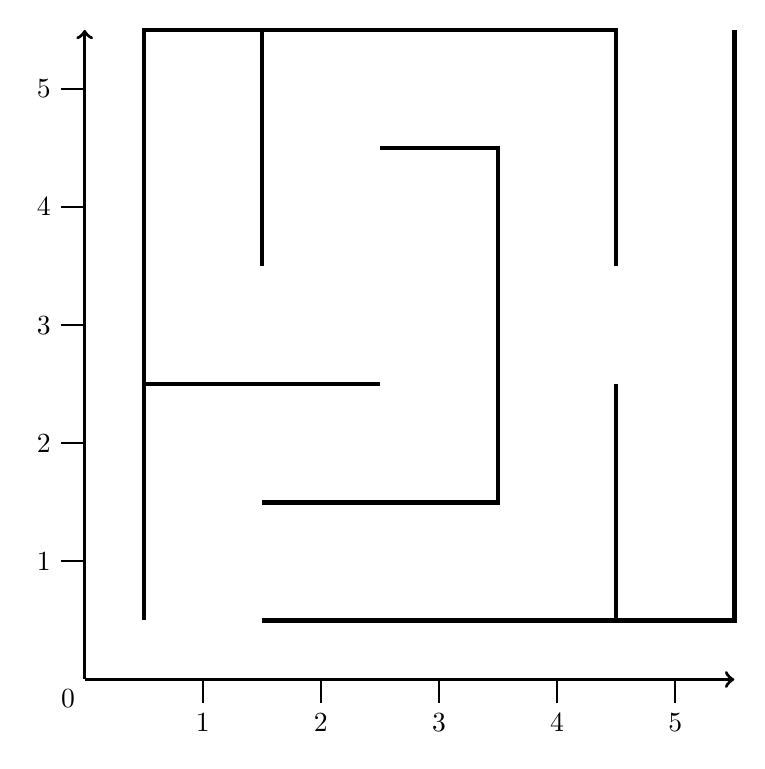
\begin{tikzpicture}[scale=1.5]
		\draw[very thick,->] (0,0) -- (5.5,0);
		\draw[very thick,->] (0,0) -- (0,5.5);
		\node[below left] at (0,0) {0};
		\foreach \x in {1,...,5} {
				\draw[thick] (\x,0) -- ++(0,-0.2) node[below] {\x};
				\draw[thick] (0,\x) -- ++(-0.2,0) node[left] {\x};
			}

		\draw[ultra thick] (0.5,0.5) -- ++(0,5) -- ++(4,0) -- ++(0,-2);
		\draw[ultra thick] (0.5,2.5) -- ++(2,0);
		\draw[ultra thick] (1.5,3.5) -- ++(0,2);
		\draw[ultra thick] (1.5,1.5) -- ++(2,0) -- ++(0,3) -- ++(-1,0);
		\draw[ultra thick] (1.5,0.5) -- ++(4,0) -- ++(0,5);
		\draw[ultra thick] (4.5,0.5) -- ++(0,2);

		% \directlua{print_path(points)}
	\end{tikzpicture}
}


\newpage

\Paste{alpha}

\end{document}